\documentclass{standalone}
\usepackage{tikz}
\usetikzlibrary{arrows.meta}

\begin{document}

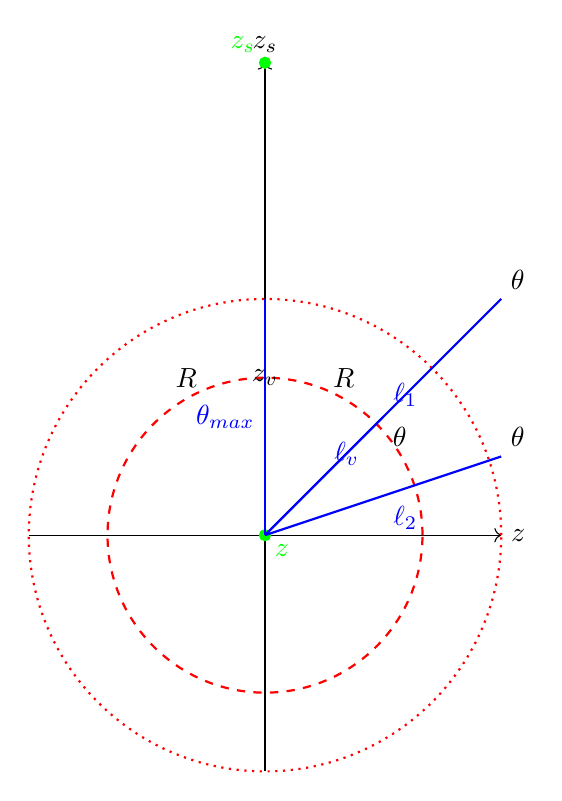
\begin{tikzpicture}[scale=2]
    % Define colors
    \definecolor{red}{RGB}{255, 0, 0}
    \definecolor{blue}{RGB}{0, 0, 255}
    \definecolor{green}{RGB}{0, 255, 0}
    
    % Draw the vertical axis
    \draw[->] (-1.5,0) -- (1.5,0) node[right] {$z$};
    \draw[->] (0,-1.5) -- (0,3) node[above] {$z_s$};
    
    % Draw the void
    \draw[dashed, thick, color=red] (0,0) circle (1);
    \draw[dotted, thick, color=red] (0,0) circle (1.5);
    
    % Draw the observer and source positions
    \filldraw[green] (0,0) circle (1pt) node[below right] {$z$};
    \filldraw[green] (0,3) circle (1pt) node[above left] {$z_s$};
    
    % Draw the photon path
    \draw[thick, color=blue] (0,0) -- (1.5,1.5) node[midway, above right] {$\ell_1$};
    \draw[thick, color=blue] (0,0) -- (1.5,0.5) node[midway, below right] {$\ell_2$};
    
    % Draw the distance from the photon's position to the center of the void
    \draw[thick, color=blue] (0,0) -- (0.75,0.75) node[midway, above right] {$\ell_v$};
    
    % Draw the maximum angle
    \draw[thick, color=blue] (0,0) -- (0,1.5) node[midway, left] {$\theta_{max}$};
    
    % Label the radius of the void
    \node at (0.5,1) {$R$};
    \node at (-0.5,1) {$R$};
    
    % Label the redshift at the center of the void
    \node at (0,1) {$z_v$};
    
    % Add labels for the angles
    \node at (0.75,0.75) [below right] {$\theta$};
    \node at (1.5,1.5) [above right] {$\theta$};
    \node at (1.5,0.5) [above right] {$\theta$};
\end{tikzpicture}

\end{document}